\documentclass[aspectratio=169]{beamer}

\usetheme{Boadilla}
\usecolortheme{beaver}
\setbeamertemplate{navigation symbols}{}
\setbeamertemplate{footline}[frame number]

\usepackage[utf8]{inputenc}
\usepackage[brazil]{babel}
\usepackage{booktabs}
\usepackage{graphicx}
\usepackage{amsmath}
\usepackage{multirow}
\usepackage{xcolor}

% Figuras geradas pelos experimentos
% Pooled (57 regiões) primeiro; região única só para os mosaicos ilustrativos.
\graphicspath{{../resultados/_pooled/}{../resultados/_pooled_blend_extra/}{../resultados/2970_3_SE/shift_consistency/}{../resultados/2970_3_SE/blend_compare/}}

\definecolor{gain}{RGB}{0,128,0}
\definecolor{loss}{RGB}{180,0,0}

\title[Invariância a Translação em SR por Tiles]{Invariância a Translação na
Super-Resolução por Tiles\\Análise do Gerador Satlas e Estratégia Ótima de Junção}
\author{Marcel Fernandes Gomes}
\institute{PPGC -- UFRGS \\ CMP620 -- Redes Neurais e Aprendizado Profundo}
\date{Junho de 2026}

% ============================================================
\begin{document}
% ============================================================

\begin{frame}
  \titlepage
\end{frame}

% ----------------------------------------------------------
\begin{frame}{Motivação: super-resolução em grandes áreas é feita por \textit{tiles}}

  \begin{columns}[T]
    \begin{column}{0.56\textwidth}
      \begin{itemize}
        \item SR por \textit{deep learning} amplia a resolução efetiva do Sentinel-2
              ($\approx$10\,m/px $\to$ $\approx$2{,}4\,m/px).
        \item Em áreas grandes, a inferência é por \textbf{tiles}: fatia-se a cena,
              super-resolve cada janela e remonta o mosaico.
        \item O modelo fixa o \emph{tamanho} do tile ($32\times32$ LR), mas a
              \emph{posição} da grade é arbitrária.
      \end{itemize}
      \begin{block}{Problema central}
        Tiles vizinhos não ``conversam'': a remontagem produz \textbf{artefatos de
        costura} nas junções.
      \end{block}
    \end{column}
    \begin{column}{0.42\textwidth}
      \centering
      
\includegraphics[width=\linewidth]{mosaic_none.png}\\
      {\small Mosaico \texttt{none}: costuras visíveis entre tiles}
    \end{column}
  \end{columns}

\end{frame}

% ----------------------------------------------------------
\begin{frame}{Pergunta de pesquisa: o gerador é invariante a translação?}

  \begin{block}{Hipótese (equivariância ideal)}
    Se o gerador $f$ fosse equivariante a translação, deslocar o conteúdo de $\Delta$
    pixels deslocaria a saída de $s\Delta$ \emph{sem mudar os valores}:
    \[
      f(T_\Delta\, x) = T_{s\Delta}\, f(x).
    \]
    Logo, dois tiles que cobrem a \emph{mesma} porção física do terreno deveriam
    produzir \textbf{os mesmos pixels} na região sobreposta.
  \end{block}

  \vspace{0.4em}
  \begin{itemize}
    \item Camadas convolucionais \emph{são} equivariantes; CNNs completas
          \textbf{não} são, por causa de \textit{padding} e subamostragem.
    \item \textbf{Conexão com a disciplina:} verificação empírica direta da
          equivariância/invariância à translação (campo receptivo, \textit{zero-padding},
          \textit{weight sharing}).
    \item Medimos \emph{quanto} essa propriedade se quebra num gerador de SR real ---
          e \emph{por quê}.
  \end{itemize}

\end{frame}

% ----------------------------------------------------------
\begin{frame}{Por que pode quebrar? Três fontes (e como as controlamos)}

  \begin{enumerate}
    \item \textbf{Campo receptivo $\gg$ tile.} \texttt{RRDBNet}: $\sim$350 convoluções
          $3\times3$ $\Rightarrow$ campo receptivo de centenas de px LR, contra um tile
          de só $32$. \emph{Todo} pixel ``vê'' a borda e o \textit{zero-padding} ---
          \textcolor{loss}{causa principal sob teste}.
    \item \textbf{Upsampling \texttt{nearest} $\times$4.} Equivariante a deslocamentos
          \emph{inteiros} em LR ($\Delta\to s\Delta$ exato). \textcolor{gain}{Por isso
          todos os deslocamentos são inteiros em px LR} --- remove o \textit{upsampling}
          como fonte de erro.
    \item \textbf{Seleção de frames.} Fixada \emph{globalmente} (uma vez,
          determinística). \textcolor{gain}{Garante que a diferença vem do modelo, não
          da entrada.}
  \end{enumerate}

  \vspace{0.5em}
  \begin{block}{Escopo do estudo}
    \emph{Zero-shot} (pesos pré-treinados \texttt{esrgan\_8S2}, sem retreino), Sentinel-2,
    8 cenas por área. Validado primeiro em \textbf{uma região} (tile MGRS T22JDM) e
    depois \textcolor{gain}{\textbf{estendido a 57 regiões}} --- resultados
    \emph{pooled} (média entre áreas).
  \end{block}

\end{frame}

% ----------------------------------------------------------
\begin{frame}{Protocolo de medida --- sem verdade de campo}

  \begin{columns}[T]
    \begin{column}{0.58\textwidth}
      \begin{enumerate}
        \item \textit{Stack} LR fixo: 8 cenas reprojetadas ao mesmo grid
              (EPSG:3857 @ 9{,}555\,m).
        \item Âncoras interiores sem \textit{nodata}.
        \item SR no \textit{offset} $0$ \emph{e} no \textit{offset} $\Delta$ ---
              $\Delta$ px LR $=s\Delta$ px HR exatos $\Rightarrow$ a sobreposição
              $\Omega$ são os \textbf{mesmos pixels físicos}.
        \item Mede-se a discordância em $\Omega$.
      \end{enumerate}
      \vspace{0.3em}
      \[
        \text{scPSNR} = 10\log_{10}\frac{255^2}{\mathrm{MSE}\big(I^{SR}_0|_\Omega,\,I^{SR}_\Delta|_\Omega\big)}
      \]
    \end{column}
    \begin{column}{0.40\textwidth}
      \begin{block}{Métrica de auto-consistência}
        Compara duas saídas SR \emph{entre si} --- \textbf{dispensa GT}.\\[0.3em]
        Reporta scPSNR, SSIM, MAE, RMSE.
      \end{block}
      \vspace{0.3em}
      \textbf{Varredura:} sobreposição de $100\%$ ($\Delta=0$, controle) a
      $\sim$$3\%$ ($\Delta=31$).
    \end{column}
  \end{columns}

\end{frame}

% ----------------------------------------------------------
\begin{frame}{Resultado 1 --- o gerador NÃO é invariante a translação}

  \begin{columns}[T]
    \begin{column}{0.46\textwidth}
      \fontsize{8pt}{10pt}\selectfont
      \begin{tabular}{cccc}
        \toprule
        \textbf{Overlap} & \textbf{scPSNR} & \textbf{SSIM} & \textbf{MAE} \\
        \midrule
        100\% (ctrl) & 99,99 & 1,000 & 0,00 \\
        90,6\% & 30,83 & 0,850 & 5,03 \\
        50,0\% & 27,81 & 0,722 & 7,99 \\
        18,8\% & 25,78 & 0,568 & 10,64 \\
        9,4\%  & 25,09 & 0,505 & 11,67 \\
        3,1\%  & 24,65 & 0,452 & 12,40 \\
        \bottomrule
      \end{tabular}

      {\fontsize{7pt}{8pt}\selectfont \emph{pooled} --- média entre 57 regiões.}
      \vspace{0.4em}
      \begin{itemize}\small
        \item Controle $\Delta=0$ $\Rightarrow$ discordância nula: protocolo validado.
        \item Queda \textbf{monotônica} ao aproximar das bordas.
        \item \textcolor{gain}{Robusto entre regiões} (dp $\pm1{,}2$\,dB).
      \end{itemize}
    \end{column}
    \begin{column}{0.52\textwidth}
      \centering
      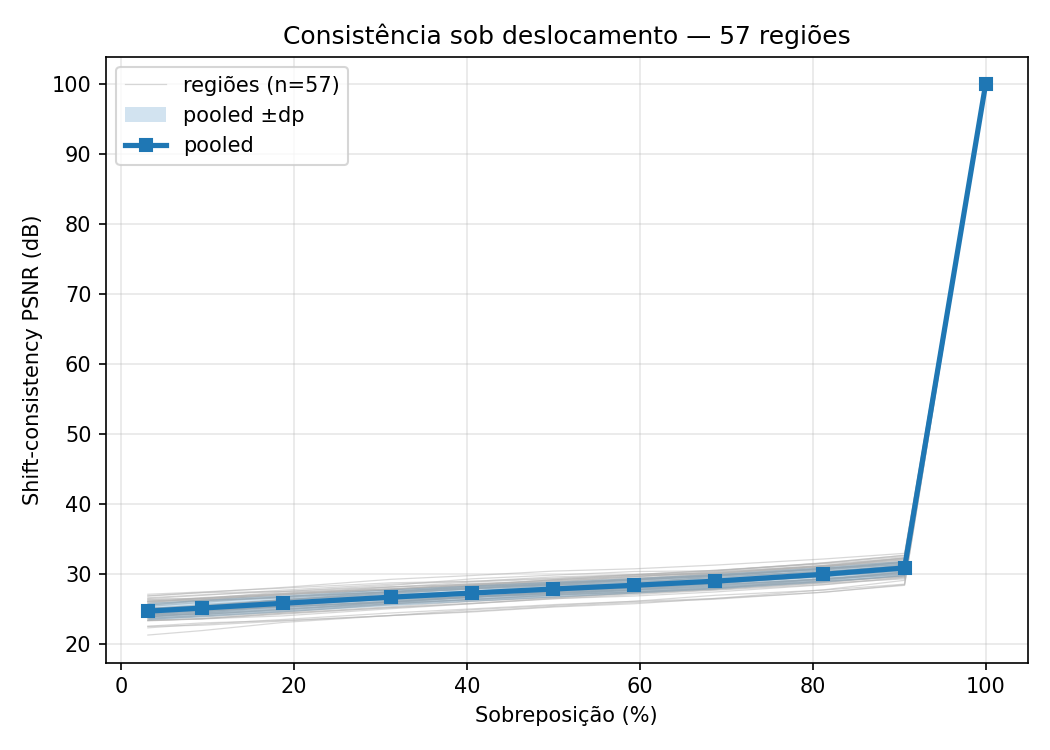
\includegraphics[width=\linewidth]{fig_consistency_pooled.png}\\
      {\small scPSNR e SSIM caem $30{,}8\to24{,}7$\,dB e $0{,}85\to0{,}45$ (57 regiões).}
    \end{column}
  \end{columns}

\end{frame}

% ----------------------------------------------------------
\begin{frame}{Resultado 2 --- onde a não-invariância se concentra}

  \begin{columns}[T]
    \begin{column}{0.5\textwidth}
      \centering
      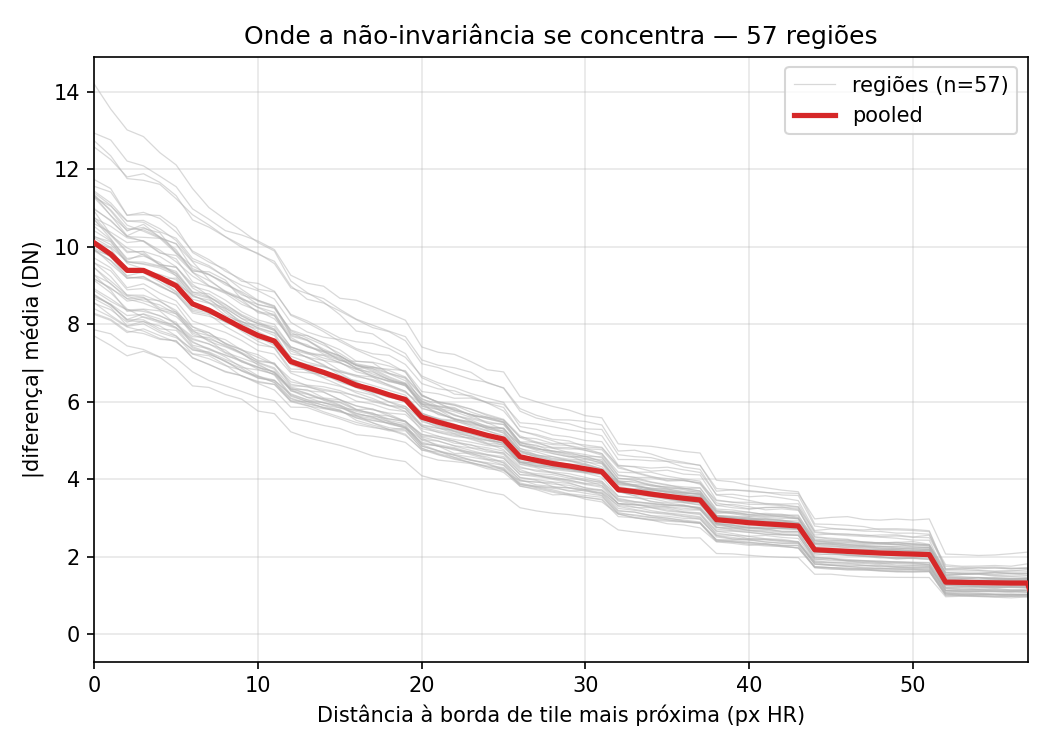
\includegraphics[width=\linewidth]{fig_border_pooled.png}
    \end{column}
    \begin{column}{0.48\textwidth}
      \begin{block}{Achado central (pooled, 57 regiões)}
        A diferença média é \textbf{máxima na borda} ($\sim$$10{,}1$\,DN) e decai para
        $\sim$$2{,}0$\,DN no interior.
      \end{block}
      \vspace{0.3em}
      \begin{itemize}
        \item Cada pixel integra o \textit{zero-padding} da borda via campo receptivo
              $\gg$ tile.
        \item O erro nasce na borda e se atenua para dentro --- exatamente como a teoria
              de equivariância prevê.
        \item O perfil é, ao mesmo tempo, a \emph{explicação} e o \emph{insumo} para a
              máscara de junção.
      \end{itemize}
    \end{column}
  \end{columns}

\end{frame}

% ----------------------------------------------------------
\begin{frame}{Resultado 3 --- qual \textit{blend} monta o mosaico sem costura?}

  \begin{columns}[T]
    \begin{column}{0.5\textwidth}
      \fontsize{8.5pt}{11pt}\selectfont
      \begin{tabular}{lccc}
        \toprule
        \textbf{Blend} & \textbf{seam}$\to$1 & \textbf{PSNR} & \textbf{SSIM} \\
        \midrule
        none        & 1,303 & 25,26 & 0,697 \\
        linear      & 1,099 & 32,03 & 0,923 \\
        cosine      & 1,072 & 33,33 & 0,945 \\
        \textcolor{gain}{\textbf{gaussian}} & \textcolor{gain}{\textbf{1,047}} & \textcolor{gain}{\textbf{34,38}} & \textcolor{gain}{\textbf{0,959}} \\
        data-driven & 1,093 & 32,41 & 0,928 \\
        \bottomrule
      \end{tabular}

      {\fontsize{7pt}{8pt}\selectfont \emph{pooled} --- média entre 57 regiões.}
      \vspace{0.3em}
      \begin{itemize}\small
        \item \texttt{none}: costura nítida ($+30\%$ de gradiente).
        \item \textbf{gaussian} vence entre as clássicas (costura \emph{e} fidelidade).
        \item Extras superam: \textbf{Poisson} (seam $0{,}98$) e \textit{data-driven
              suavizado} (PSNR $34{,}9$).
      \end{itemize}
    \end{column}
    \begin{column}{0.48\textwidth}
      \centering
      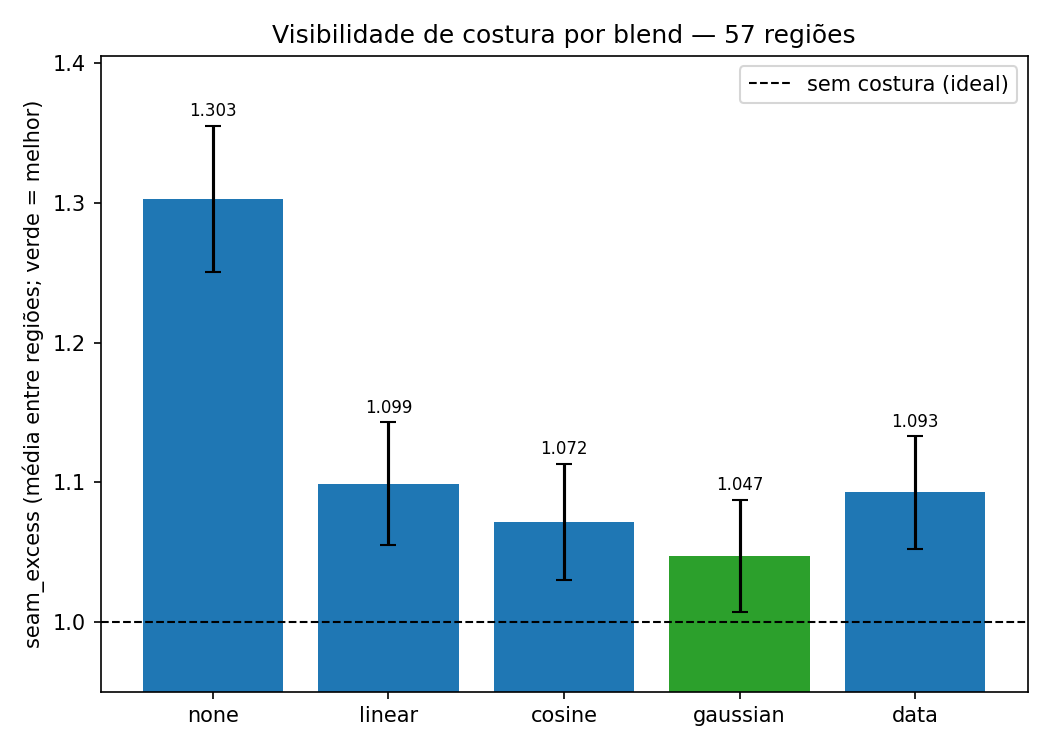
\includegraphics[width=\linewidth]{fig_blend_pooled.png}\\
      {\small \texttt{seam\_excess}: ideal $=1{,}0$ (tracejado).}
    \end{column}
  \end{columns}

\end{frame}

% ----------------------------------------------------------
\begin{frame}{Recomendação prática de montagem}

  \begin{block}{Como remontar mosaicos sem costura}
    \begin{enumerate}
      \item Usar \textbf{sobreposição não-nula} entre tiles vizinhos.
      \item Aplicar \textbf{\textit{feathering} gaussiano} na transição.
      \item \textbf{Descartar as bordas} onde o erro de equivariância é máximo
            (faixa de $\sim$15--20\,px HR).
    \end{enumerate}
  \end{block}

  \vspace{0.5em}
  \begin{columns}[T]
    \begin{column}{0.48\textwidth}
      \centering
      
\includegraphics[width=\linewidth]{mosaic_none.png}\\
      {\small \texttt{none} --- costuras}
    \end{column}
    \begin{column}{0.48\textwidth}
      \centering
      
\includegraphics[width=\linewidth]{mosaic_gaussian.png}\\
      {\small \texttt{gaussian} --- sem costura}
    \end{column}
  \end{columns}

\end{frame}

% ----------------------------------------------------------
\begin{frame}{Conclusão e trabalhos futuros}

  \begin{block}{Resposta à pergunta central}
    \textbf{Não:} o gerador Satlas/ESRGAN não é invariante a translação. A discordância
    cresce $30{,}8\to24{,}7$\,dB ao aproximar das bordas, e a causa é o
    \textit{zero-padding} sob um campo receptivo maior que o tile.
  \end{block}

  \vspace{0.3em}
  \textbf{Contribuições:}
  \begin{enumerate}
    \item Protocolo de \textit{shift-consistency} \textbf{sem GT}.
    \item Diagnóstico do efeito de borda (campo receptivo $\gg$ tile).
    \item \textit{Blend} gaussiano reduz costura $1{,}30\to1{,}05$ e eleva PSNR a
          $34{,}4$\,dB (extras Poisson/suavizado superam).
    \item \textcolor{gain}{\textbf{Validação \emph{pooled} em 57 regiões}}: achado
          robusto, com baixa dispersão entre áreas.
  \end{enumerate}

  \vspace{0.3em}
  \textbf{Trabalhos futuros:}
  \begin{itemize}
    \item Consolidar junção em \textbf{domínio de gradiente} (Poisson/Dirichlet) e
          máscaras \textit{data-driven} suavizadas como sucessoras da gaussiana.
    \item \textit{Anti-aliasing} no gerador; \textit{finetuning} com perda de
          consistência de borda $\mathcal{L}_{borda}$.
  \end{itemize}

\end{frame}

% ----------------------------------------------------------
\begin{frame}[plain]
  \begin{block}{Mensagem central}
    A equivariância \emph{formal} das camadas convolucionais não se traduz em
    invariância \emph{prática} num gerador de SR profundo: o \textit{zero-padding},
    amplificado por um campo receptivo que excede o tile, quebra a consistência entre
    posições. Medir esse efeito sem GT e ponderá-lo com um \textit{blend} adequado
    basta para montar mosaicos sem costura.
  \end{block}
  \vspace{3em}
  \begin{center}
    \Large\textbf{Obrigado!}\\[0.6em]
    \normalsize marcelgfernandes@gmail.com
  \end{center}
\end{frame}

% ============================================================
\end{document}
